\documentclass[aspectratio=169,10pt]{beamer}
\usepackage[T1]{fontenc}
\usepackage[utf8]{inputenc}
\usepackage{amsmath,graphicx,xcolor}
\usepackage{tikz}
\usetikzlibrary{arrows.meta,positioning}
\graphicspath{{figures/}{../docs/screenshots/}}

\definecolor{navy}{HTML}{1F4E79}
\definecolor{teal}{HTML}{1B7F79}
\definecolor{warm}{HTML}{B5651D}
\definecolor{soft}{HTML}{EAF1F8}
\definecolor{muted}{HTML}{5A6572}

\usetheme{default}
\usefonttheme{professionalfonts}
\setbeamertemplate{navigation symbols}{}
\setbeamercolor{structure}{fg=navy}
\setbeamercolor{itemize item}{fg=teal}
\setbeamercolor{block title}{bg=navy,fg=white}
\setbeamercolor{block body}{bg=soft,fg=black}
\setbeamerfont{frametitle}{series=\bfseries,size=\Large}
\setbeamertemplate{frametitle}{%
  \vskip3mm\hskip-0.5mm\usebeamercolor[fg]{frametitle}\usebeamerfont{frametitle}\insertframetitle\par
  \vskip1mm{\color{navy}\hrule height 0.8pt}\vskip2mm}
\setbeamertemplate{footline}{%
  \hfill{\color{muted}\scriptsize\insertframenumber/\inserttotalframenumber}\hspace{4mm}\vskip3mm}

\newcommand{\hl}[1]{{\color{warm}\bfseries #1}}
\newcommand{\ui}[1]{\texttt{\color{navy}#1}}

\tikzset{
  box/.style={draw=navy,fill=soft,rounded corners=2pt,align=center,minimum height=10mm,inner sep=4pt},
  hw/.style={box,fill=warm!15,draw=warm},
  arr/.style={-{Stealth[length=2.5mm]},navy,very thick}
}

\begin{document}

% ------------------------------------------------------------------ 1
\begin{frame}[plain]
  \vspace{12mm}
  \begin{center}
    {\color{navy}\huge\bfseries PCA of ToF-SIMS spectra}\\[3mm]
    {\color{teal}\Large All-peak PCA and Selected-peak PCA}\\[8mm]
    {\normalsize Jose Tupayachi \quad$\cdot$\quad Oak Ridge National Laboratory}\\[1mm]
    {\color{muted}\small \today}
  \end{center}
\end{frame}

% ------------------------------------------------------------------ 2
\begin{frame}{What PCA does}
  \begin{columns}[T]
    \begin{column}{0.56\textwidth}
      \begin{itemize}\setlength\itemsep{4mm}\large
        \item A sample is a spectrum: hundreds of numbers (here \hl{901 bins}).
        \item PCA finds a few new axes, \hl{PC1}, \hl{PC2}, \ldots, that keep as much of the difference between samples as possible.
        \item Samples with similar spectra end up \hl{close together} on the map.
      \end{itemize}
      \vspace{3mm}
      \begin{block}{Two things to read}
        \hl{Scores}: one dot per sample.\\
        \hl{Loadings}: which peaks pull each axis.
      \end{block}
    \end{column}
    \begin{column}{0.4\textwidth}
      \begin{center}
      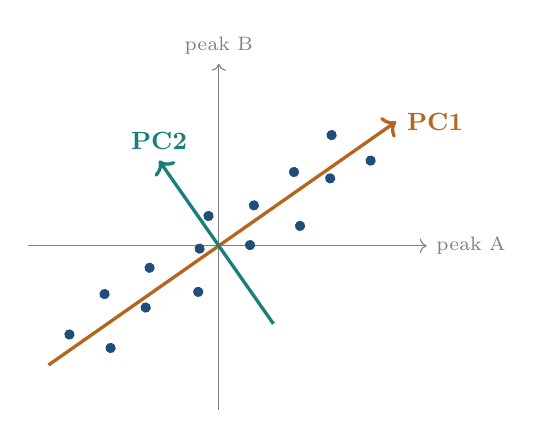
\begin{tikzpicture}[scale=1.1]
        \draw[->,gray] (-2.2,0) -- (2.4,0) node[right,font=\scriptsize] {peak A};
        \draw[->,gray] (0,-1.9) -- (0,2.1) node[above,font=\scriptsize] {peak B};
        \begin{scope}[rotate=35]
          \foreach \u/\v in {-2/0.15,-1.7/-0.25,-1.4/0.3,-1.1/-0.1,-0.8/0.25,-0.5/-0.3,-0.2/0.1,0.1/0.35,0.3/-0.2,0.6/0.15,0.9/-0.35,1.2/0.2,1.5/-0.1,1.8/0.3,2.0/-0.2}
            \fill[navy] (\u,\v) circle (1.7pt);
          \draw[->,warm,very thick] (-2.4,0) -- (2.5,0) node[right,font=\small\bfseries,warm] {PC1};
          \draw[->,teal,very thick] (0,-1.1) -- (0,1.2) node[above,font=\small\bfseries,teal] {PC2};
        \end{scope}
      \end{tikzpicture}\\[-1mm]
      {\scriptsize PC1 follows the longest direction of the cloud}
      \end{center}
    \end{column}
  \end{columns}
\end{frame}

% ------------------------------------------------------------------ 3
\begin{frame}{Transformations: the settings in the interface}
  \begin{columns}[T]
    \begin{column}{0.47\textwidth}
      \fbox{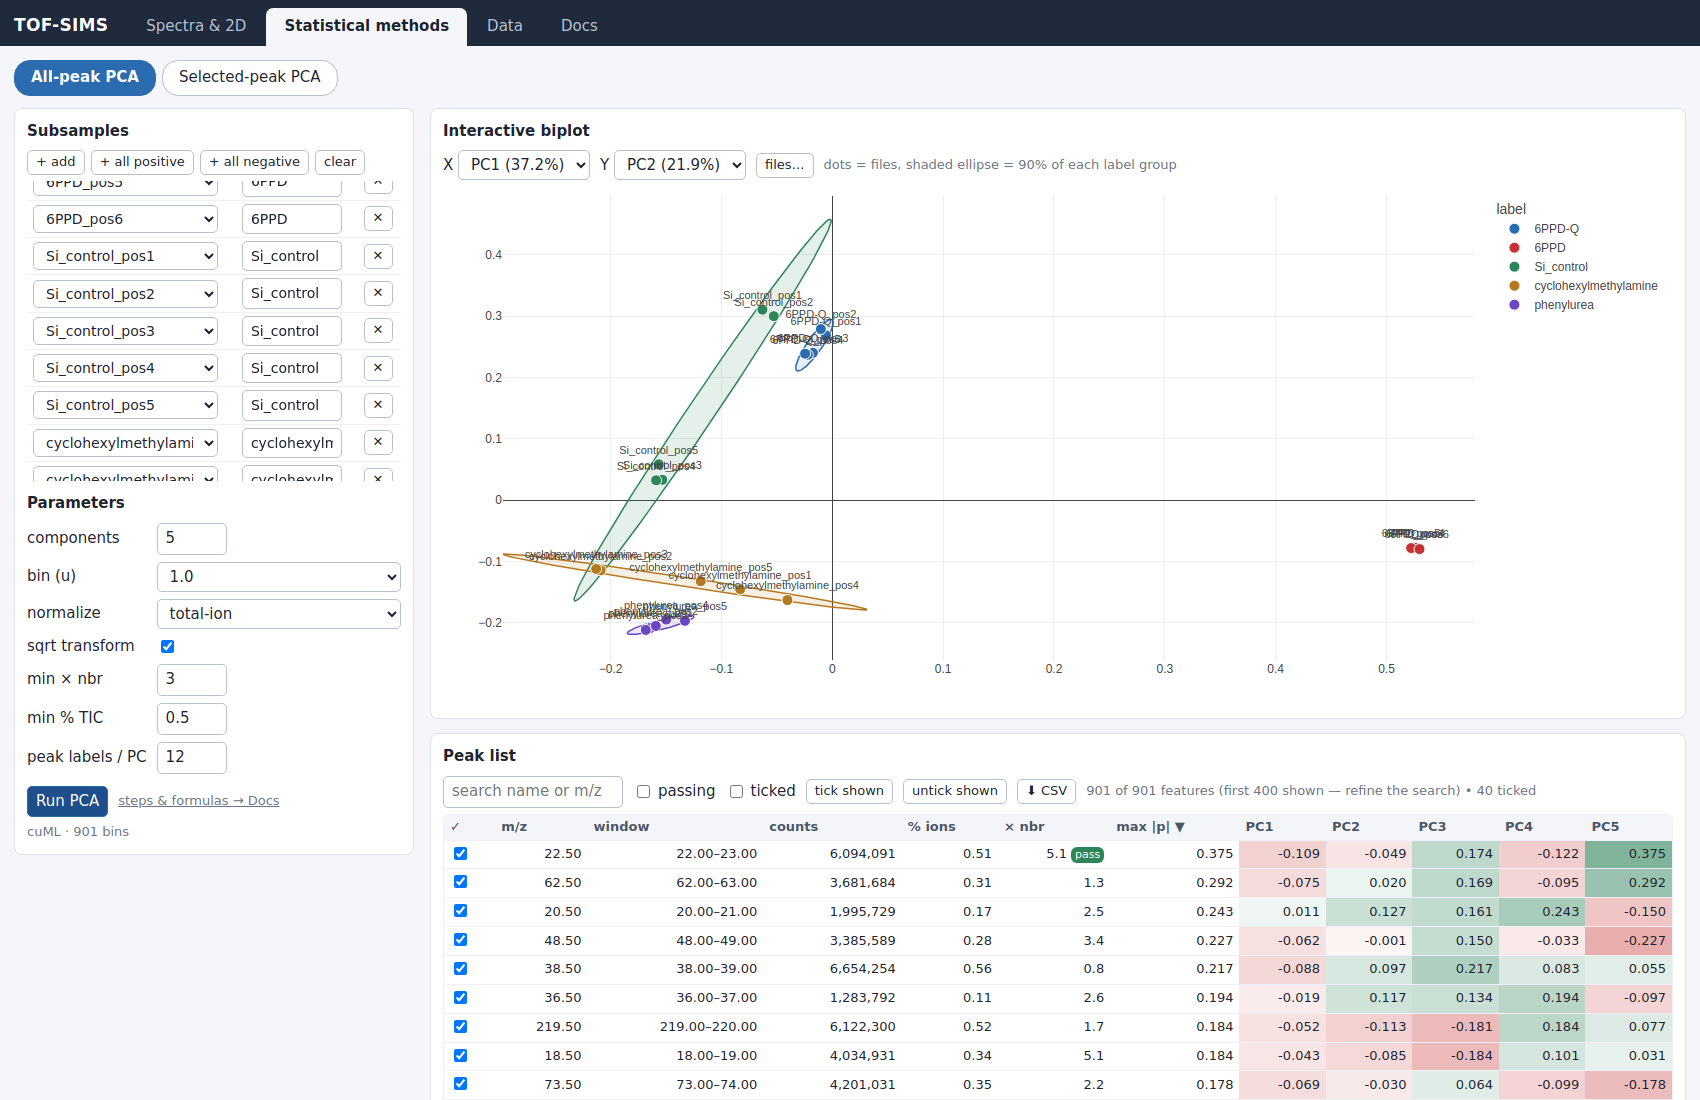
\includegraphics[trim=14bp 250bp 1285bp 488bp,clip,width=\textwidth]{04_pca.png}}\\[-1mm]
      {\scriptsize \textit{Statistical methods} tab, parameters panel}
    \end{column}
    \begin{column}{0.51\textwidth}
      \begin{itemize}\setlength\itemsep{2.4mm}
        \item \ui{bin (u)}: width of each m/z bin. One bin = one variable.
        \item \ui{normalize = total-ion}: divide each spectrum by its own total, $x/\sum x$. Removes differences in total signal.
        \item \ui{sqrt transform}: take $\sqrt{x}$. Shrinks the big peaks and evens out counting noise.
        \item \hl{Mean centring} is always applied: subtract the average spectrum.
        \item \ui{components}: how many PCs to compute.
      \end{itemize}
      \vspace{1mm}
      \centering\hl{normalise $\rightarrow$ $\sqrt{\ }$ $\rightarrow$ centre $\rightarrow$ PCA}
    \end{column}
  \end{columns}
\end{frame}

% ------------------------------------------------------------------ 4
\begin{frame}{Two rounds of PCA (Yang et al.\ 2019)}
  \centering
  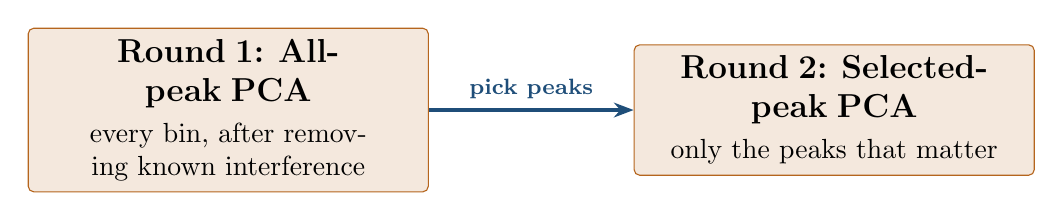
\begin{tikzpicture}
    \node[hw,text width=4.8cm] (a) {\large\textbf{Round 1: All-peak PCA}\\[1mm]\normalsize every bin, after removing known interference};
    \node[hw,text width=4.8cm,right=26mm of a] (b) {\large\textbf{Round 2: Selected-peak PCA}\\[1mm]\normalsize only the peaks that matter};
    \draw[arr] (a) -- node[above,font=\footnotesize\bfseries,navy] {pick peaks} (b);
  \end{tikzpicture}
  \vspace{3mm}
  \begin{itemize}\setlength\itemsep{2mm}\large
    \item All-peak PCA: strong matrix peaks (in Yang's study, culture-medium salts) dominate the result.
    \item Selected-peak PCA: peaks dominated by the medium are dropped, characteristic ones are kept. The same samples separate, and the \hl{loadings are easier to interpret}.
    \item Rule of thumb for round 2 (Fu et al.\ 2018): a peak is at least \hl{3$\times$} its neighbours and holds more than \hl{0.5\%} of the ions. These are \ui{min $\times$ nbr} and \ui{min \% TIC} in the interface.
  \end{itemize}
  \vfill
  {\scriptsize Yang et al., \textit{Biointerphases} 14, 051004 (2019). \quad Fu et al., \textit{Atmos.\ Environ.} 191, 36 (2018).}
\end{frame}

% ------------------------------------------------------------------ 5
\begin{frame}{In the interface: from All-peak to Selected-peak}
  \begin{columns}[T]
    \begin{column}{0.44\textwidth}
      \begin{enumerate}\setlength\itemsep{2.2mm}
        \item Pick subsamples and labels, click \ui{Run PCA} on the \hl{All-peak PCA} tab.
        \item The \ui{Peak list} ranks every bin by its influence on the PCs. The 40 strongest are pre-ticked. \ui{pass} marks bins that meet the 3$\times$ and 0.5\% rule.
        \item Tick or untick peaks.
        \item Open the \hl{Selected-peak PCA} tab: the same transformations, only on the ticked peaks.
      \end{enumerate}
    \end{column}
    \begin{column}{0.54\textwidth}
      \fbox{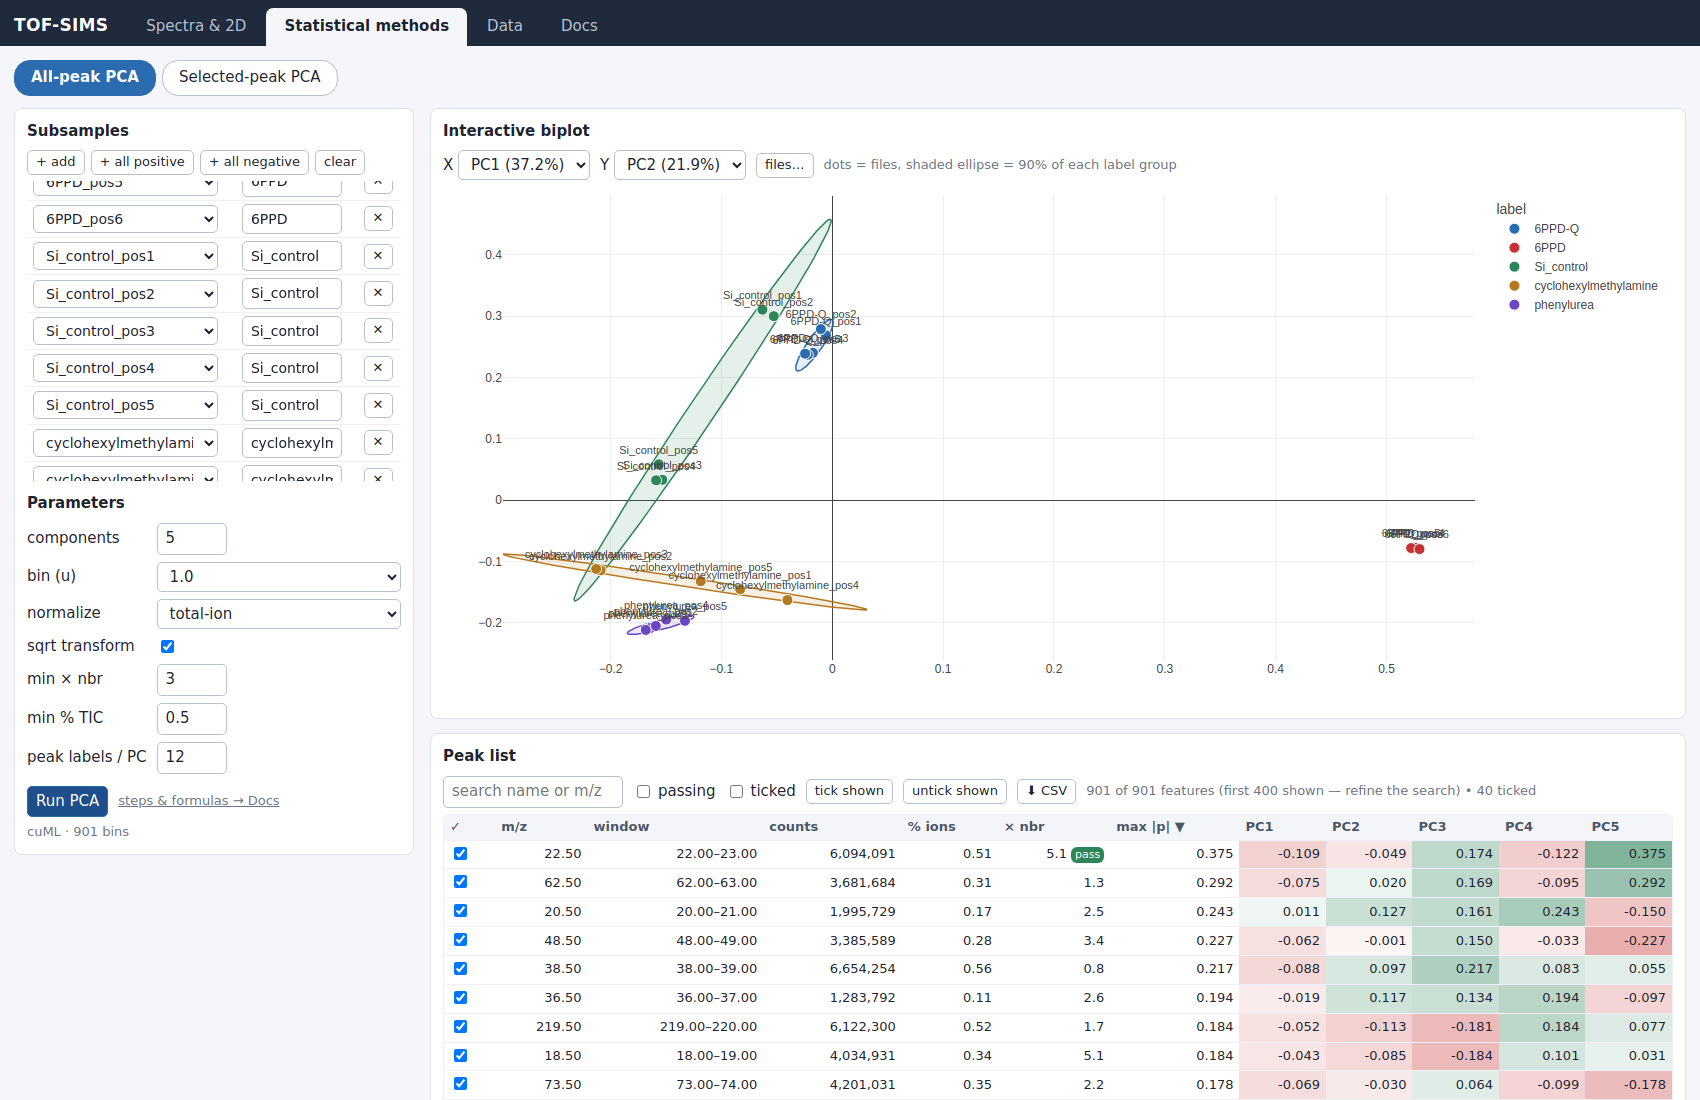
\includegraphics[trim=14bp 1002bp 1360bp 58bp,clip,width=0.62\textwidth]{04_pca.png}}\\[2mm]
      \fbox{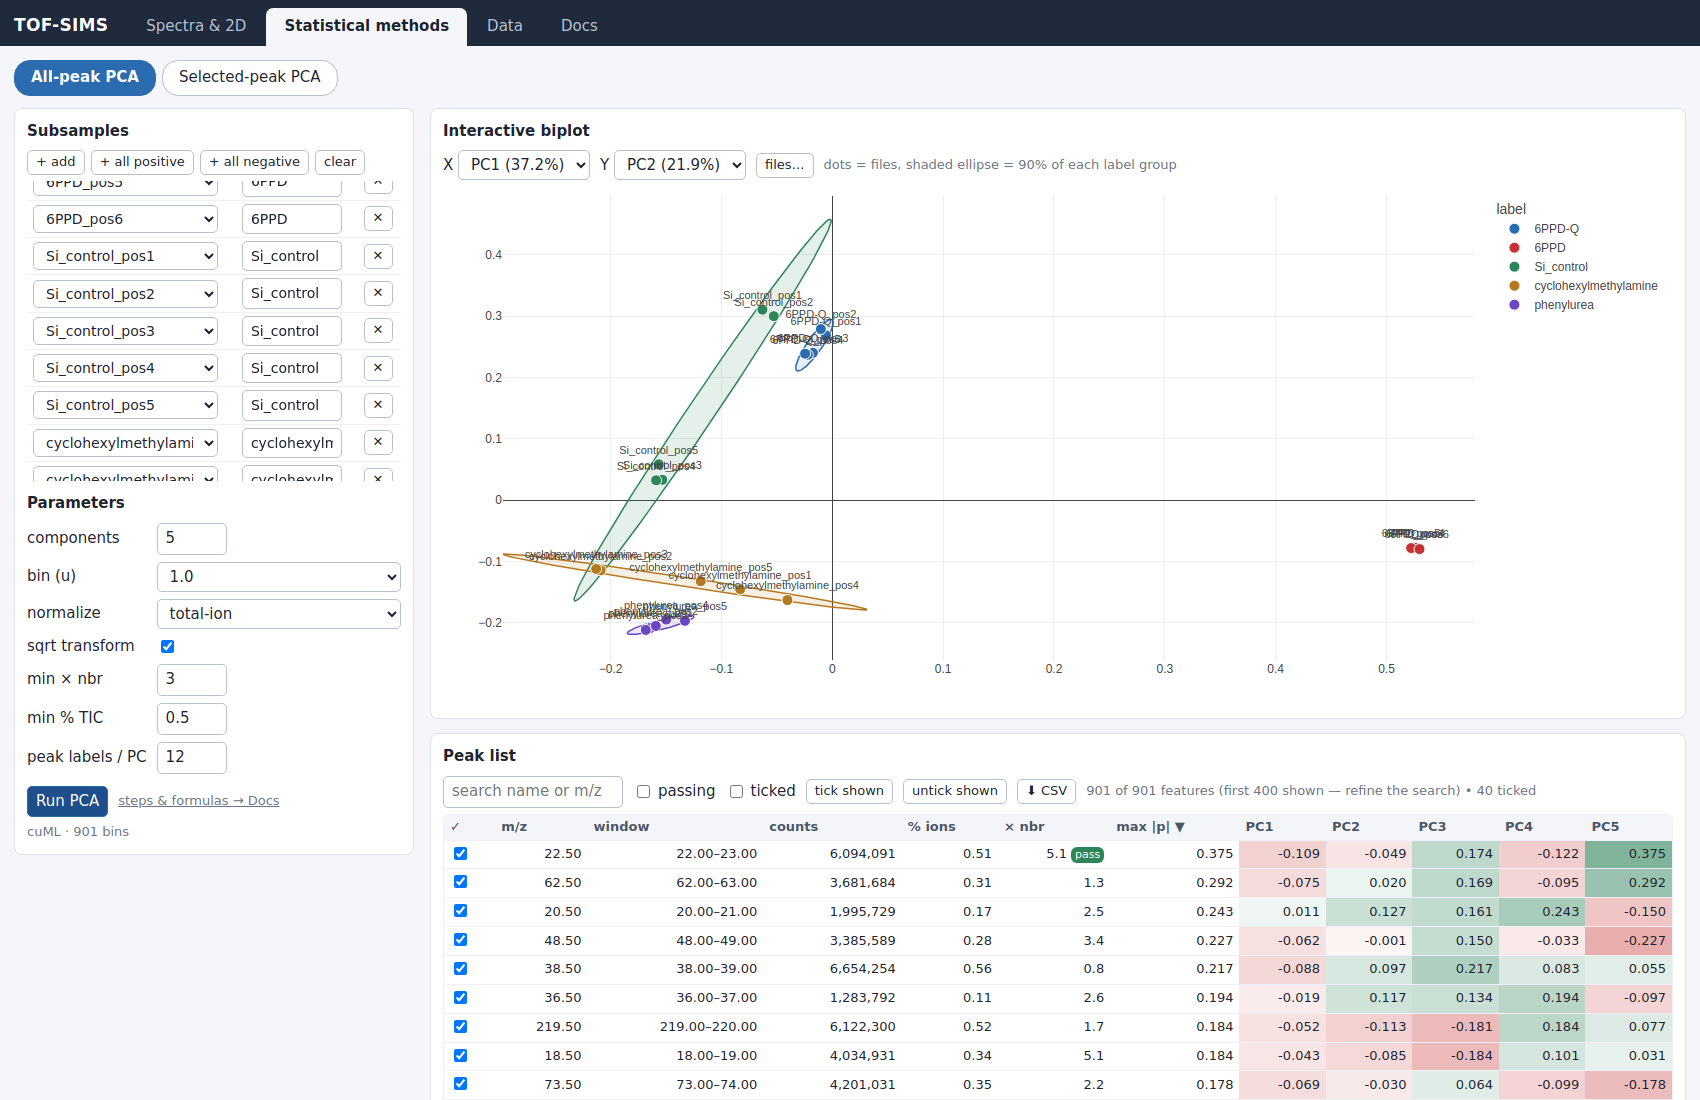
\includegraphics[trim=443bp 0bp 460bp 770bp,clip,width=\textwidth]{04_pca.png}}\\[-1mm]
      {\scriptsize Peak list: ticked peaks, m/z, share of ions, \texttimes\ neighbour, pass, loadings}
    \end{column}
  \end{columns}
  \vfill
  {\scriptsize Not in the tool: removal of PDMS and Bi primary ions, and Yang's medium-overlay filter.}
\end{frame}

% ------------------------------------------------------------------ 6
\begin{frame}{Real data: the two PCAs side by side}
  \begin{columns}[T]
    \begin{column}{0.46\textwidth}
      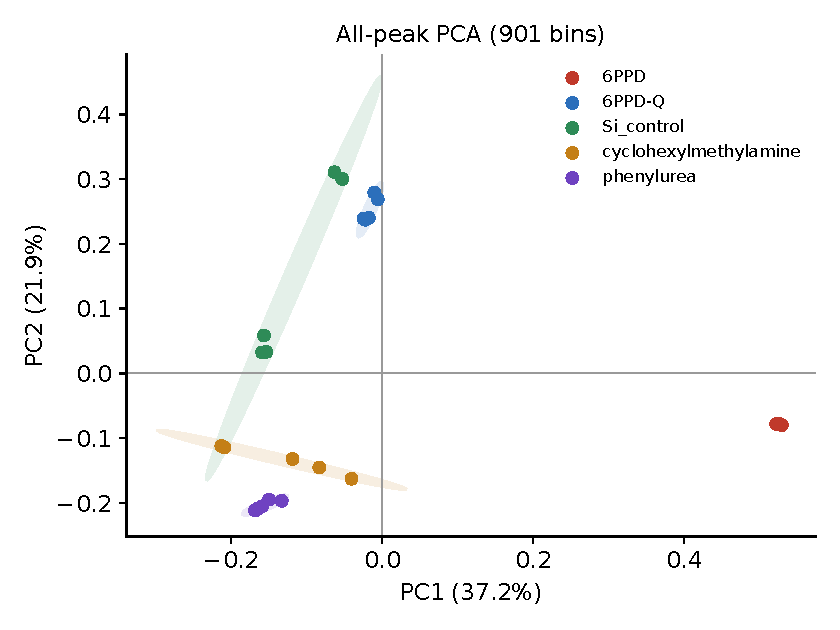
\includegraphics[width=\textwidth]{scores_all.pdf}
    \end{column}
    \begin{column}{0.46\textwidth}
      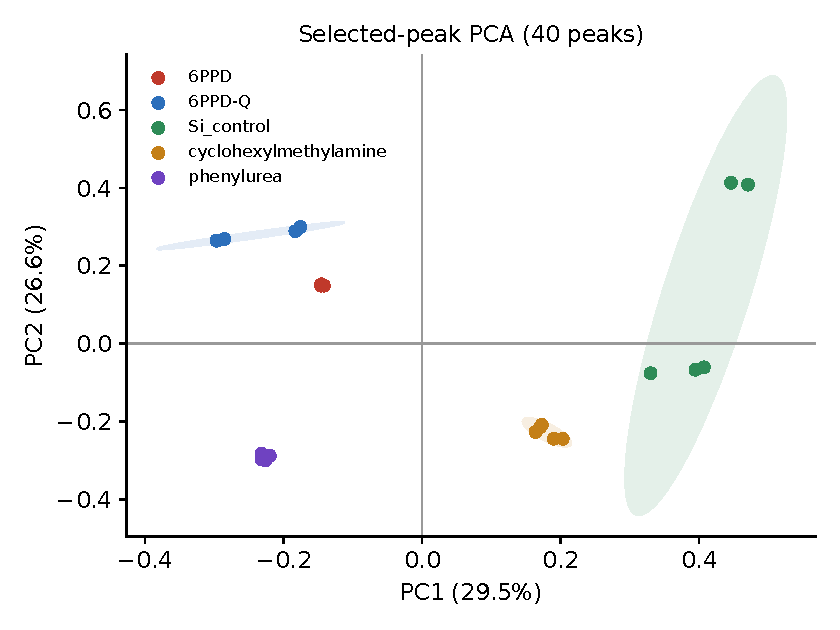
\includegraphics[width=\textwidth]{scores_sel.pdf}
    \end{column}
  \end{columns}
  \vspace{1mm}
  \begin{itemize}\setlength\itemsep{1.5mm}
    \item 24 positive-polarity subsamples, five groups. Same transformations in both.
    \item PC1 + PC2 explain \hl{59.1\%} (901 bins) and \hl{56.1\%} (40 peaks).
    \item The 40 peaks are picked from the same data, so the separation is \hl{descriptive}, not a test.
  \end{itemize}
\end{frame}

\end{document}
